\documentclass[tikz,border=8pt]{standalone}
\usepackage[scaled=0.95]{helvet}
\renewcommand{\familydefault}{\sfdefault}
\usepackage{amsmath}
\usepackage{xcolor}
\definecolor{TEJNavy}{HTML}{1E2B55}
\definecolor{TEJOrange}{HTML}{E97828}
\definecolor{TEJRule}{HTML}{B8C2D1}
\begin{document}
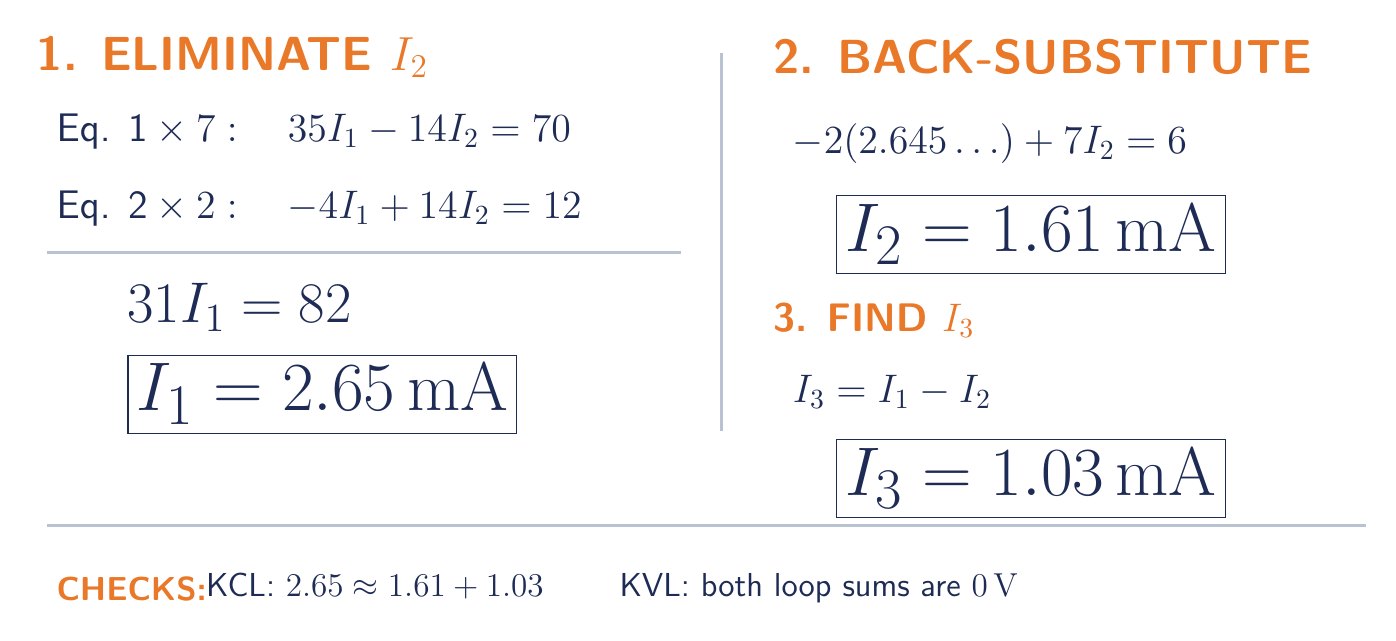
\begin{tikzpicture}[text=TEJNavy]
  \node[anchor=west,font=\bfseries\LARGE,text=TEJOrange] at (0,6.3)
    {1. ELIMINATE $I_2$};
  \node[anchor=west,font=\Large] at (0.25,5.35)
    {$\text{Eq. 1}\times 7:\quad 35I_1-14I_2=70$};
  \node[anchor=west,font=\Large] at (0.25,4.38)
    {$\text{Eq. 2}\times 2:\quad -4I_1+14I_2=12$};
  \draw[TEJRule,line width=1.2pt] (0.25,3.82) -- (8.3,3.82);
  \node[anchor=west,font=\huge] at (1.15,3.12) {$31I_1=82$};
  \node[anchor=west,font=\Huge] at (1.15,2.02)
    {$\boxed{I_1=2.65\,\mathrm{mA}}$};

  \draw[TEJRule,line width=1.2pt] (8.82,1.55) -- (8.82,6.35);

  \node[anchor=west,font=\bfseries\LARGE,text=TEJOrange] at (9.35,6.3)
    {2. BACK-SUBSTITUTE};
  \node[anchor=west,font=\Large] at (9.60,5.20)
    {$-2(2.645\ldots)+7I_2=6$};
  \node[anchor=west,font=\Huge] at (10.15,4.05)
    {$\boxed{I_2=1.61\,\mathrm{mA}}$};
  \node[anchor=west,font=\bfseries\Large,text=TEJOrange] at (9.35,2.95)
    {3. FIND $I_3$};
  \node[anchor=west,font=\Large] at (9.60,2.05) {$I_3=I_1-I_2$};
  \node[anchor=west,font=\Huge] at (10.15,0.95)
    {$\boxed{I_3=1.03\,\mathrm{mA}}$};

  \draw[TEJRule,line width=1.2pt] (0.25,0.35) -- (17.0,0.35);
  \node[anchor=west,font=\bfseries\large,text=TEJOrange] at (0.25,-0.45) {CHECKS:};
  \node[anchor=west,font=\large] at (2.15,-0.45)
    {KCL: $2.65\approx1.61+1.03$ \qquad KVL: both loop sums are $0\,\mathrm{V}$};
\end{tikzpicture}
\end{document}
